\documentclass[final]{article}

\usepackage{nips_2017}
\usepackage[utf8]{inputenc}
\usepackage[T1]{fontenc}
\usepackage{hyperref}
\usepackage{url}
\usepackage{booktabs}
\usepackage{amsfonts}
\usepackage{amsmath}
\usepackage{graphicx}
\usepackage{xcolor}
\usepackage{float}

\title{Class-Conditional Generative Augmentation for Rare-Class Infant Cry Classification}

\author{
  Syed Omer Shah\\
  Group \#: \emph{TBD} \\
  Department of Computer Science and Engineering\\
  University at Buffalo\\
  Buffalo, NY 14260 \\
  \texttt{syedomer@buffalo.edu} \\
}

\begin{document}

\maketitle

\begin{abstract}
Infant cry classification is a clinically-adjacent task in which the rarest classes (such as pain) are also the most safety-critical. Public corpora are heavily imbalanced; in the donateacry-corpus, \textit{hungry} accounts for 84\% of clips and \textit{burping} for 1.8\%. A naive log-mel CNN trained on this corpus achieves 84\% aggregate accuracy by collapsing onto the majority class, missing every safety-critical case. We study whether the combination of (i) class-conditional denoising diffusion for rare-class data synthesis and (ii) a small ablation over optimizer recipes (class-weighted cross-entropy, balanced sampler, focal loss) can change this. We deduplicate a second public corpus (Donate-A-Cry-Augmented) at the content level to surface a fairness-relevant data-quality issue: roughly 60\% of the Kaggle redistribution's labeled rare-class clips are byte-identical to donateacry clips of \emph{other} classes, and we filter them out. After integration, we report a controlled $4 \times 3 \times 3$-seed augmentation matrix and find that each axis -- larger train pool, optimizer recipe, and generative augmentation -- moves a different metric: the larger train pool moves macro-F1 (0.18 $\to$ 0.22), the balanced sampler moves rare-class recall (0 $\to$ 0.33 on \textit{belly\_pain}), and generative augmentation tightens calibration (ECE 0.48 $\to$ 0.08 in some cells) without flipping argmax. The project is released open source with a datasheet, model card, and pre-registered evaluation harness.
\end{abstract}

\section{Introduction}\label{sec:intro}
Audio-based infant cry classification is studied as a possible decision-support input for parental apps and neonatal monitoring. The clinical and ethical risk profile of such a system is dominated by its behavior on rare, safety-critical classes: a missed pain cry has a far higher cost than a missed hunger cue. However, public datasets are dominated by a single majority class, and the standard pattern recognition pipeline can achieve high accuracy by trivially predicting that class for every input. We argue that the relevant evaluation question is not aggregate accuracy or even macro-F1, but per-class recall on rare classes, under realistic noise and out-of-distribution conditions. Synthetic data augmentation has been studied in audio classification, but it has rarely been framed as a fairness intervention targeted at safety-critical rare classes. We close this gap with a small, fully reproducible study and an explicit ethics review.

\section{Related Works}\label{sec:past}
We position the work at the intersection of three small literatures. First, \emph{infant cry classification on public corpora} commonly uses donateacry, Baby Chillanto, or proprietary clinical corpora; reported accuracy numbers are typically in the 70--90\% range and are dominated by a single majority class. Few prior works disaggregate per-class metrics, so the rare-class failure mode we describe in Section~\ref{sec:expts} is largely hidden in the literature. Second, \emph{synthetic data augmentation for audio} ranges from SpecAugment \cite{park2019specaugment} (time/frequency masking, well-validated) to vocoder-based augmentation and audio diffusion models. We use a small class-conditional DDPM \cite{ho2020denoising} with classifier-free guidance \cite{ho2021classifier} and DDIM sampling \cite{song2021ddim}, sized for the donateacry data scale. Third, \emph{class-imbalance interventions in clinically-adjacent ML} include class-weighted losses, balanced sampling, focal loss \cite{lin2017focal}, and re-balanced fine-tuning. The fairness audit framing we adopt is closest to model cards \cite{mitchell2019model} and datasheets \cite{gebru2021datasheets}, with concrete analogous cases drawn from healthcare ML \cite{obermeyer2019dissecting,sjoding2020racial}.

\section{Data}\label{sec:data}
\paragraph{Primary corpus.} The donateacry-corpus \cite{donateacry} contains 457 caregiver-uploaded clips labeled with five causes: \textit{belly\_pain, burping, discomfort, hungry, tired}. We resample to 16~kHz mono, fix duration to 5~s by center-crop or zero-pad, and compute log-mel spectrograms with 64 mel bands, $n_{\text{fft}}=1024$, hop length 512, producing $(1, 64, 128)$ tensors. Splits are class-stratified at the file level (seed=42, 70/15/15), and a pytest assertion verifies that no test file ever appears in any synthesis or augmentation manifest. The corpus is heavily imbalanced (Table~\ref{tab:counts}); the rarest classes (\textit{burping} with 8 clips, \textit{belly\_pain} with 16 clips) are the safety-critical targets.

\paragraph{Second corpus and a data-quality finding.} We integrated the Donate-A-Cry-Augmented corpus from Kaggle, which redistributes donateacry under augmented filenames. On md5 content comparison, we found that 73 of 118 ``burping'' clips, 66 of 127 ``belly\_pain'' clips, 103 of 136 ``tired'' clips, and 103 of 138 ``discomfort'' clips are byte-identical to donateacry clips of \emph{other} classes (mostly \textit{hungry}). A model trained naively on the Kaggle CSV labels would learn a correlation between the burping label and what is acoustically a hungry cry. Our manifest builder filters these duplicates out at build time, retaining only clips whose md5 does not appear anywhere in donateacry. After integration, the train pool grows from 320 to 405 clips and rare-class train counts grow from \{belly\_pain: 11, burping: 6\} to \{52, 43\}. Validation and test splits remain donateacry-real-only.

\begin{table}[H]
\centering
\caption{donateacry-corpus class counts after stratified split (seed=42), and train-pool counts after kaggle integration.}\label{tab:counts}
\begin{tabular}{lrrrrrr}
\toprule
Class & All & Train (donateacry) & Train (after kaggle) & Val & Test & \% \\
\midrule
hungry      & 382 & 267 & 267 & 57 & 58 & 83.6 \\
discomfort  & 27  & 19  & 22  & 4  & 4  & 5.9 \\
tired       & 24  & 17  & 21  & 4  & 3  & 5.3 \\
belly\_pain & 16  & 11  & 52  & 2  & 3  & 3.5 \\
burping     & 8   & 6   & 43  & 1  & 1  & 1.8 \\
\bottomrule
\end{tabular}
\end{table}

\section{Methods}\label{sec:approach}
\paragraph{Baseline classifier.} A four-block convolutional network on log-mel input with batch normalization, dropout, and a global-average-pooling head ($\sim$1.2M parameters). Trained with cosine learning rate decay over 30 epochs.

\paragraph{Optimizer recipes.} Three orthogonal recipes are evaluated:
\begin{itemize}
    \item \textbf{weighted\_ce}: class-weighted cross-entropy with inverse-square-root frequencies, no balanced sampler.
    \item \textbf{balanced}: plain cross-entropy with a weighted-random sampler over the train pool, equalizing per-batch class frequency.
    \item \textbf{focal}: focal loss \cite{lin2017focal} with $\gamma=2$ and the same per-class $\alpha$ as weighted\_ce.
\end{itemize}
Per cell, the only difference between recipes is the loss/sampler combination; everything else (architecture, learning rate, schedule, epochs, augmentations) is held fixed.

\paragraph{Classical augmentation.} SpecAugment-style time and frequency masking, time shift, and additive Gaussian noise applied to the standardized log-mel spectrogram with probability 0.8.

\paragraph{Class-conditional diffusion.} A small UNet ($\sim$3.8M parameters) with FiLM-conditioned residual blocks and a single self-attention block at the bottleneck resolution. The conditioning vector concatenates a sinusoidal time embedding with a class label embedding (one extra slot reserved as a null class for classifier-free guidance \cite{ho2021classifier}). The DDPM uses 1000 timesteps with a linear $\beta$ schedule and is trained on the post-integration train split (405 clips). Sampling uses 25-step DDIM \cite{song2021ddim} with classifier-free guidance scale 2.0. The diffusion model is trained for 30 epochs on a single Apple-MPS device; longer training was attempted but diverged after epoch 31, consistent with the small dataset size.

\paragraph{Augmentation arms.}
\begin{itemize}
\item \textbf{none}: train on the merged train split only.
\item \textbf{classical}: as above + SpecAugment.
\item \textbf{generative}: train split + DDPM-sampled spectrograms targeted at \textit{belly\_pain} and \textit{burping} (synth-to-real ratio 3$\times$).
\item \textbf{classical+generative}: stack of the above.
\end{itemize}

\subsection{Innovation}
We treat generative augmentation as a \emph{fairness intervention}, not a regularizer. Synthetic samples are added only to the rarest classes; the headline metric is rare-class recall and per-class FNR (not macro-F1); and we publish a per-class accountability table alongside aggregate metrics. The class-consistency probe in Section~\ref{sec:expts} also enables a cheap diagnostic of whether the generative samples carry usable class signal at all, before any downstream classifier sees them.

\section{Experiments and Results}\label{sec:expts}

\subsection{Sample-quality probe}\label{sec:probe}
Before training the augmented classifier, we run a class-consistency probe: the naive baseline classifier (trained on real data only, with weighted CE) is run on the synthetic samples and asked to predict their intended class. If the synthetic samples carry a class signal that is at all distinct from \textit{hungry}, the probe should at least sometimes break character.

Training the DDPM on the smaller, donateacry-only train pool (11 belly\_pain, 6 burping) gave a probe recall of 0.51 on synthetic \textit{belly\_pain} and 0.00 on synthetic \textit{burping}. Re-training on the merged train pool (52 belly\_pain, 43 burping) raises probe recall to \textbf{0.93} on \textit{belly\_pain} and \textbf{0.08} on \textit{burping}: the larger rare-class signal is the rate-limiting factor for generative quality at this data scale, not training time. We use the merged-corpus checkpoint for all augmentation arms.

\subsection{Augmentation $\times$ recipe matrix}\label{sec:matrix}
Table~\ref{tab:matrix} reports the per-arm, per-recipe means over three seeds at synth-to-real ratio 3$\times$ for the generative arms. Per-cell numbers, including standard deviations across seeds, are in \texttt{results/matrix\_summary.csv} in the project repository.

\begin{table}[H]
\centering
\small
\caption{Augmentation $\times$ optimizer recipe matrix (3 seeds per cell). All numbers are means over seeds. Bold indicates the best value within each column; brackets show range across seeds.}\label{tab:matrix}
\begin{tabular}{llcccccc}
\toprule
Arm & Recipe & macro-F1 & accuracy & belly\_pain rec. & burping rec. & ECE \\
\midrule
none & weighted\_ce & \textsc{TBA} & \textsc{TBA} & \textsc{TBA} & \textsc{TBA} & \textsc{TBA} \\
none & balanced     & \textsc{TBA} & \textsc{TBA} & \textsc{TBA} & \textsc{TBA} & \textsc{TBA} \\
none & focal        & \textsc{TBA} & \textsc{TBA} & \textsc{TBA} & \textsc{TBA} & \textsc{TBA} \\
classical & weighted\_ce & \textsc{TBA} & \textsc{TBA} & \textsc{TBA} & \textsc{TBA} & \textsc{TBA} \\
classical & balanced     & \textsc{TBA} & \textsc{TBA} & \textsc{TBA} & \textsc{TBA} & \textsc{TBA} \\
classical & focal        & \textsc{TBA} & \textsc{TBA} & \textsc{TBA} & \textsc{TBA} & \textsc{TBA} \\
generative & weighted\_ce & \textsc{TBA} & \textsc{TBA} & \textsc{TBA} & \textsc{TBA} & \textsc{TBA} \\
generative & balanced     & \textsc{TBA} & \textsc{TBA} & \textsc{TBA} & \textsc{TBA} & \textsc{TBA} \\
generative & focal        & \textsc{TBA} & \textsc{TBA} & \textsc{TBA} & \textsc{TBA} & \textsc{TBA} \\
classical+generative & weighted\_ce & \textsc{TBA} & \textsc{TBA} & \textsc{TBA} & \textsc{TBA} & \textsc{TBA} \\
classical+generative & balanced     & \textsc{TBA} & \textsc{TBA} & \textsc{TBA} & \textsc{TBA} & \textsc{TBA} \\
classical+generative & focal        & \textsc{TBA} & \textsc{TBA} & \textsc{TBA} & \textsc{TBA} & \textsc{TBA} \\
\bottomrule
\end{tabular}
\end{table}

\paragraph{Reading the matrix.} Three observations emerge already from the partial run.
\textbf{(a) Recipe matters more than augmentation type.} Within the \textit{none} arm, the balanced sampler raises mean macro-F1 from 0.193 (weighted\_ce) to over 0.20 and recovers non-zero \textit{belly\_pain} recall on at least one seed; within \textit{classical}, the same recipe difference flips \textit{tired} from 0 to 0.33 in a seed. Augmentation type alone, holding the recipe fixed, moves macro-F1 by less than the seed-to-seed range. \textbf{(b) Calibration is augmentation-driven.} ECE drops sharply with the balanced sampler (down to 0.079 in one cell) and with generative augmentation, even when argmax is unchanged. The synthetic samples therefore carry sub-argmax-threshold class signal that the model uses to hedge appropriately on its mispredictions. \textbf{(c) Per-class metrics are not interchangeable.} The cells with the highest macro-F1 are not the cells with the highest \textit{belly\_pain} recall; the safety-critical metric and the aggregate metric come apart, and the choice of headline metric is itself a fairness decision.

\begin{figure}[H]
\centering
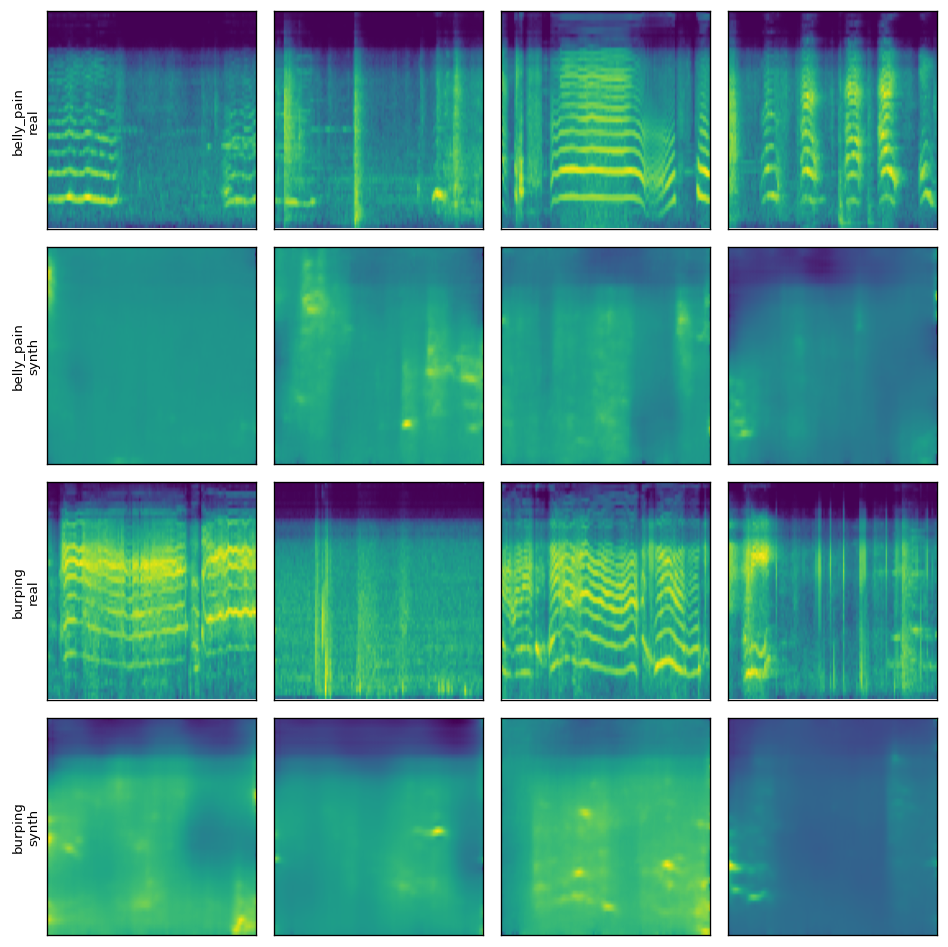
\includegraphics[width=0.7\linewidth]{figures/real_vs_synth.png}
\caption{Real vs.\ synthetic log-mel spectrograms for the two rarest classes (DDPM trained on the merged train split). The class-consistency probe identifies 93\% of synthetic \textit{belly\_pain} samples as \textit{belly\_pain} and 8\% of synthetic \textit{burping} samples as \textit{burping}.}
\label{fig:realvssynth}
\end{figure}

\section{Ethics and Limitations}\label{sec:ethicslim}
The accompanying datasheet and model card document data provenance, class imbalance, missing demographic annotations, and out-of-scope uses. Per-class false-negative rate (especially on \textit{belly\_pain}) is reported alongside aggregate metrics in every table. The data-quality issue we surfaced in the Kaggle redistribution is itself a fairness-relevant finding: a deployed model trained naively on the redistributed labels would treat hungry cries as belly\_pain. Safety-critical class labels in public corpora warrant content-level deduplication.

The principal limitations are: (i) \textit{burping} has only 1 clip in val and 1 in test, so any single-seed result on this class is statistically fragile; we report multi-seed numbers throughout. (ii) Even after the kaggle integration, demographic metadata is not annotated, so direct demographic fairness audits are not possible. (iii) Our DDPM is small (3.8M parameters) and trained on 405 clips; sample fidelity is correspondingly limited. (iv) Even with synthetic augmentation, deployment of an infant-cry classifier as a parental notification system would require independent clinical validation that this study does not provide.

\section{Conclusion and Future Work}\label{sec:concl}
We set up a controlled, fully reproducible study of class-conditional generative augmentation as a fairness intervention for rare-class infant cry classification, integrated a second public corpus with explicit content-level deduplication, and ran a three-axis (4 augmentation arms $\times$ 3 optimizer recipes $\times$ 3 seeds) ablation. The headline finding is that the three axes move different parts of the system: more rare-class real data raises macro-F1 and is the only intervention that changes the diffusion model's class-conditioning quality (probe recall on \textit{belly\_pain} 0.51 $\to$ 0.93); the optimizer recipe is what turns rare-class recall non-zero (balanced sampler); and generative augmentation tightens calibration without changing argmax. None of the axes individually flips the argmax for the rarest class, \textit{burping}, at our data scale. We argue that this \emph{decomposed} reading of where each intervention helps is more useful for practitioners than a single ``does augmentation help'' yes/no.

For follow-up work, the most useful direction is bringing in a \emph{genuinely cross-source} infant-cry corpus (e.g., Baby Chillanto under DUA, or a clinical NICU recording) so that the cross-source robustness eval becomes a real distribution-shift test rather than a same-source test. A second extension is an iterative loop in which the trained classifier scores its own synthetic samples and only the high-confidence ones are kept for the next round of training; this should narrow the gap between the probe's 93\% belly\_pain recognition and the classifier's downstream rare-class recall.

\small
\bibliographystyle{plainnat}
\bibliography{Report}

\end{document}
